% Created 2025-04-29 Tue 19:45
% Intended LaTeX compiler: pdflatex
\documentclass[11pt]{article}
\usepackage[utf8]{inputenc}
\usepackage[T1]{fontenc}
\usepackage{graphicx}
\usepackage{longtable}
\usepackage{wrapfig}
\usepackage{rotating}
\usepackage[normalem]{ulem}
\usepackage{amsmath}
\usepackage{amssymb}
\usepackage{capt-of}
\usepackage{hyperref}
\usepackage{minted}
\usepackage{pgfplots, graphicx, siunitx}
\graphicspath{ {./images/} }
\author{Hankertrix}
\date{\today}
\title{Math Module 2B Notes}
\hypersetup{
 pdfauthor={Hankertrix},
 pdftitle={Math Module 2B Notes},
 pdfkeywords={},
 pdfsubject={},
 pdfcreator={Emacs 30.1 (Org mode 9.7.11)}, 
 pdflang={English}}
\begin{document}

\maketitle
\setcounter{tocdepth}{2}
\tableofcontents \clearpage\section{Definitions}
\label{sec:org4d08b1f}

\subsection{Derivative}
\label{sec:org10c1c8d}
Given a function \(f(x)\), it's \textbf{derivative} at a point \(a\) is:
\[f'(a) = \lim_{h \rightarrow 0} \frac{f(a + h) - f(a)}{h}\]

If the above limit exists, then we say the function \(f\) is \textbf{differentiable} at the point \(a\). Also, when we say that the derivative \(f'(a)\) \textbf{exists}, we mean that the limit above exists (it's a real number), which means \(f\) is differentiable at \(a\).


By putting \(x = a + h\), we can rewrite the expression as:
\[f'(a) = \lim_{x \rightarrow a} \frac{f(x) - f(a)}{x - a}\]
\subsubsection{Notation for the set of functions differentiable at \(x = a\)}
\label{sec:org97b2505}
The set of functions differentiable at \(x = a\) is denoted by \(D(a)\), so if we write \(f \in D(a)\), it means that the limit \(f'(a)\) exists.
\subsubsection{Interpretation}
\label{sec:orgce7f12b}
In the sciences, derivative means \textbf{rate of change}.

\textbf{Example}: If \(s(t)\) is the distance travelled (\(\unit{m}\)) at time \(t\) (\(\unit{s}\)), then \(s'(t)\) is the velocity (\(\unit{m.s^{-1}}\)) at time \(t\) and \(s''(t)\) is the acceleration (\(\unit{m.s^{-2}}\)) at time \(t\).


\textbf{Example}: If \(Q(t)\) is the amount of charge (\(\unit{C}\)) that's passed through a cross-section of a wire at time \(t\) (\(\unit{s}\)), then \(Q'(t)\) is the current \(A\) (\(\unit{C.s^{-1}}\))

\newpage
\subsection{Powers of x}
\label{sec:org1f0c5cb}
\[x^r = e^{r \ln x}\]
\subsection{Unit circle}
\label{sec:org2209f3e}
A unit circle is a circle with \textbf{radius 1} and is \textbf{centred} at the \textbf{origin}.
\subsection{\(\cos \theta\) and \(\sin \theta\) for arbitrary \(\theta \in \mathbb{R}\)}
\label{sec:org87072a7}
Let \(\theta in \mathbb{R}\) and consider the point \((x, y)\) on the \textbf{unit circle} whose angle with the positive \(x\)-axis is \(\theta\) (counterclockwise for \(\theta > 0\), clockwise for \(\theta < 0\)). We define:
\[\cos \theta = x, \quad \sin \theta = y\]

\[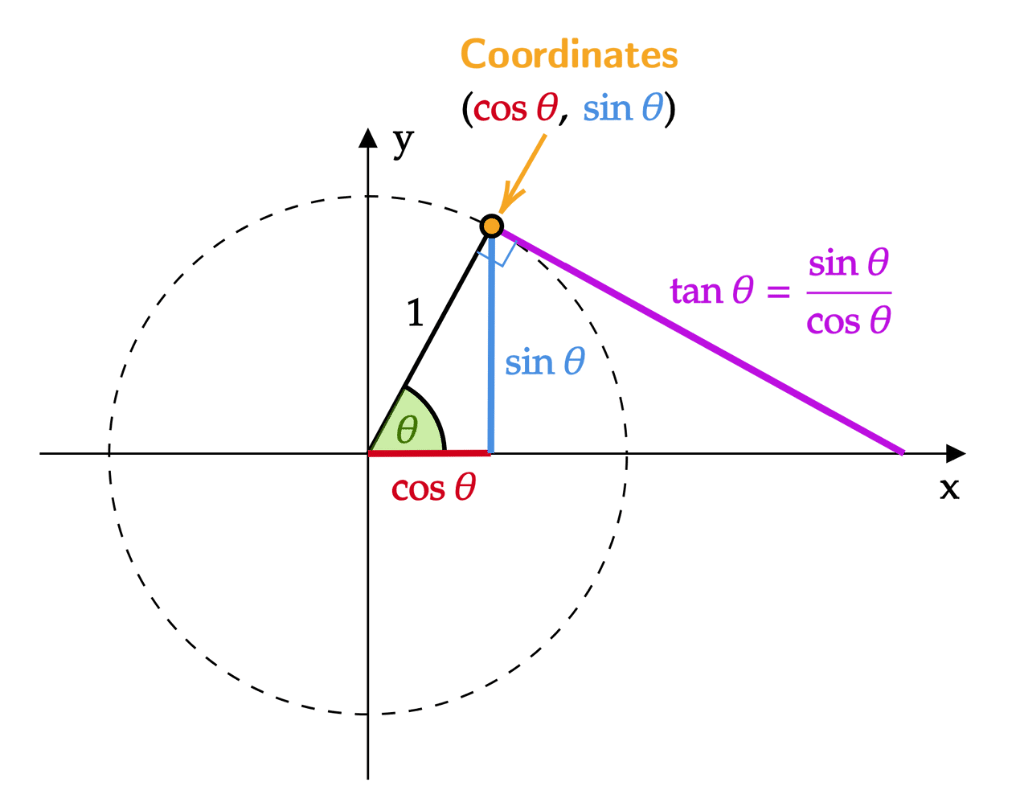
\includegraphics[width = \textwidth]{unit-circle}\]
\subsection{Global maximum}
\label{sec:orgdd2766c}
Consider a function \(f : A \rightarrow \mathbb{R}\). A point \(x_0 \in A\) is called a \textbf{point of global maximum} if:
\[f(x) \le f(x_0), \quad \text{for all } x \in A\]
\subsection{Global minimum}
\label{sec:orgedf0508}
Consider a function \(f : A \rightarrow \mathbb{R}\). A point \(x_0 \in A\) is called a \textbf{point of global minimum} if:
\[f(x) \ge f(x_0), \quad \text{for all } x \in A\]
\subsection{Local maximum}
\label{sec:orgfe4b1d3}
Consider a function \(f : A \rightarrow \mathbb{R}\). A point \(x_0 \in A\) is called a \textbf{point of local maximum} if there exists some open interval \((a, b) \ni x_0\) such that:
\[f(x) \le f(x_0), \quad \text{for all } x \in (a, b) \cap A\]
\subsection{Local minimum}
\label{sec:org3f27cab}
Consider a function \(f : A \rightarrow \mathbb{R}\). A point \(x_0 \in A\) is called a \textbf{point of local minimum} if there exists some open interval \((a, b) \ni x_0\) such that:
\[f(x) \ge f(x_0), \quad \text{for all } x \in (a, b) \cap A\]
\subsection{Critical point}
\label{sec:org98a4630}
A \textbf{critical point} of a function \(f : A \rightarrow \mathbb{R}\) is \(c \in A\) such that either \(f'(c) = 0\) or \(f'(c)\) does not exist.
\subsection{Extremum}
\label{sec:org08a6a51}
Extremum just means the maximum or minimum value of a function.

\newpage
\section{Derivative as the slope of the tangent}
\label{sec:orgf3c80f0}
Let \(f(x)\) be a function that is differentiable at \(x = a\). The line passing through the points \((a, f(a))\) and \((a + h, f(a + h))\) on \(f\)'s graph, is given by:
\[y = \frac{f(a + h) - f(a)}{h} (x - a) + f(a)\]

As \(h\) tends to 0, this line approaches the \textbf{tangent line} at \((a, f(a))\).
\[\text{Slope of the line} = \frac{\Delta y}{\Delta x} = \frac{f(a + h) - f(a)}{h}\]

The limit of the line is \(f'(a)\) as \(h \rightarrow 0\). Hence, \(f'(a)\) is the slope of the tangent.


The equation for the tangent line would be:
\[y = f'(a) \cdot (x - a) + f(a)\]

This equation only makes sense if \(f'(a)\) is a finite real number, which means \(f \in D(a)\).


For an interactive graph illustrating the derivative as the slope of the tangent, go to \href{https://www.desmos.com/calculator/gdn4qknq1w}{this link.}

\newpage
\section{Differentiability implies continuity}
\label{sec:org4805536}
If a function \(f\) is differentiable at a point \(a\), then \(f\) is also continuous at the point \(a\). That means that \(D(a) \subset C(a)\).


\textbf{Proof}:


Suppose \(f\) is differentiable at \(a\), which means:
\[\lim_{h \rightarrow 0} \frac{f(a + h) - f(a)} = f'(a) \text{ exists}\]

Then:
\begin{align*}
\lim_{x \rightarrow a} f(x) &= \lim_{h \rightarrow 0} \frac{f(a+h) - f(a)}{h} \cdot h + f(a) \\
&= f'(a) \cdot 0 + f(a) \\
&= f(a)
\end{align*}

We just proved:
\[f \text{ differentiable at } x = a \Rightarrow f \text{ continuous at } x = a\]
\subsection{Contrapositive form}
\label{sec:org90550a7}
This theorem is most often used in its contrapositive form:


If \(f\) is \textbf{not continuous} at \(x = a\), then it is also \textbf{not differentiable} at \(x = a\).

\newpage
\subsection{The reverse does not hold true}
\label{sec:orgeff6c05}
\(f\) being continuous at \(x = a\) does \textbf{not} mean that \(f\) is differentiable at \(x = a\).
\subsubsection{Example 1}
\label{sec:org54ea906}
Let \(f(x) = \sqrt[3]{x}\):


\(f(x)\) is continuous at \(x = 0\) as it is an elementary function, but is it differentiable at \(x = 0\)?
\begin{align*}
\lim_{h \rightarrow 0} \frac{f(0 + h) - f(0)}{h} &= \lim_{h \rightarrow 0} \frac{h^{\frac{1}{3}} - 0}{h} \\
&= \lim_{h \rightarrow 0} h^{-\frac{2}{3}} \\
&= \lim_{h \rightarrow 0} \frac{1}{h^{\frac{2}{3}}} \\
&= + \infty
\end{align*}

Hence, \(\lim_{h \rightarrow 0} f(x)\) does not exist, and thus \(f\) is \textbf{not} differentiable at \(x = 0\).


\begin{center}
\begin{tikzpicture}
\begin{axis}[axis lines = center]
\addplot[domain=-10:10, samples=100, color=blue]{x/abs(x)*abs(x)^(1/3)};
\addplot[color=red] coordinates {(0, -2) (0, 2)};
\end{axis}
\end{tikzpicture}
\end{center}

The graph of \(f(x) = \sqrt[3]{x}\) has a vertical tangent at \((0, 0)\), which means it is \textbf{not} differentiable at \((0, 0)\).

\newpage
\subsubsection{Example 2}
\label{sec:org9ab06cf}
Let \(f(x) = \sin |x|\):


\(f(x)\) is continuous at \(x = 0\) as it is an elementary function, but is it differentiable at \(x = 0\)?

\begin{align*}
\lim_{h \rightarrow 0} \frac{f(0 + h) - f(0)}{h} &= \lim_{h \rightarrow 0} \frac{\sin |h| - \sin |0|}{h} \\
&= \lim_{h \rightarrow 0} \frac{\sin |h|}{h}
\end{align*}

Getting the left-hand limit:
\begin{align*}
\lim_{h \rightarrow 0-} \frac{\sin |h|}{h} &= \lim_{h \rightarrow 0-} \frac{\sin (-h)}{h} \\
&= \frac{- \sin h}{h} \\
&= -1
\end{align*}

Getting the right-hand limit:
\begin{align*}
\lim_{h \rightarrow 0+} \frac{\sin |h|}{h} &= \lim_{h \rightarrow 0+} \frac{\sin (h)}{h} \\
&= \frac{\sin h}{h} \\
&= 1
\end{align*}

\newpage

\begin{center}
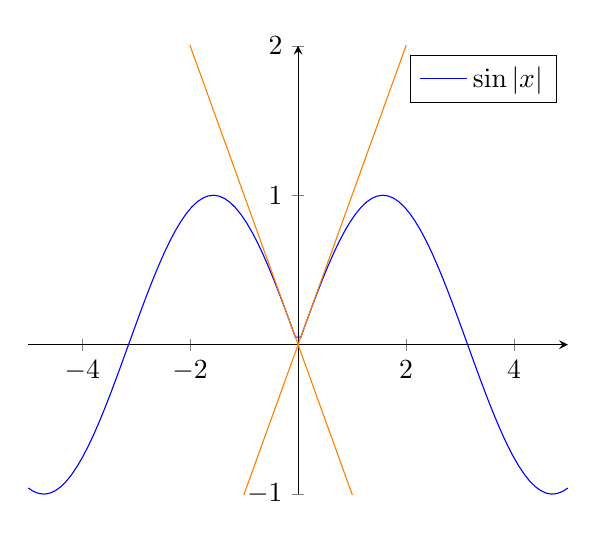
\begin{tikzpicture}
\begin{axis}[axis lines = center, ymin = -1, ymax = 2]
\addplot[color=blue, samples = 100]{sin(abs(deg(x)))};
\addlegendentry{\(\sin |x|\)}
\addplot[color=orange]{x};
\addplot[color=orange]{-x};
\end{axis}
\end{tikzpicture}
\end{center}

Since \(\lim_{h \rightarrow 0-} \frac{\sin |h|}{h} \neq \lim_{h \rightarrow 0+} \frac{\sin |h|}{h}\), \(\lim_{h \rightarrow 0} \frac{\sin |h|}{h}\) does not exist and thus, \(f\) is not differentiable at 0.

\newpage
\section{Differentiation rules}
\label{sec:org0b579bd}
Given two functions \(f\) and \(g\), and given that the right-hand side makes sense, we have:

\begin{enumerate}
\item Sum rule, for any real constants \(c, d\): \((cf + dg)'(x) = cf'(x) + dg'(x)\)
\item Product rule: \((fg)'(x) = f'(x)g(x) + f(x)g'(x)\)
\item Ratio rule (Quotient rule): \(\left( \frac{f}{g} \right)'(x) = \frac{f'(x)g(x) - f(x) g'(x)}{(g(x))^2}\)
\item Chain rule: \([f(g(x))]' = f'(g(x)) \cdot g'(x)\)
\end{enumerate}

Note the condition that the right-hand side must make sense for the equation to hold, which means the \textbf{derivative} for \(f\) and \(g\) \textbf{must exist}. In particular, the theorem tells us that:
\begin{itemize}
\item If \(f\) and \(g\) are both differentiable at \(x\), then so is \(cf + dg\).
\item If \(f\) and \(g\) are both differentiable at \(x\), then so is \(fg\).
\item If \(f\) and \(g\) are both differentiable at \(x\) and \(g(x) \neq 0\), then \(\frac{f}{g}\) is differentiable at \(x\).
\item If \(g\) is differentiable at \(x\) and \(f\) is differentiable at \(g(x)\), then \(f(g(x))\) is differentiable at \(x\).
\end{itemize}

If the right-hand side does not make sense, then the theorem gives us \textbf{no information}.

\newpage
\subsection{Example 1}
\label{sec:org52924c2}
If \(f(x) = x \sin x\), what is \(f'(x)\)?

\[f'(x) = 1 \cdot \sin x + x \cdot \cos x\]

In particular, since both \(x\) and \(\cos x\) are differentiable, the product rule tells us that \(x \cdot \sin x\) is differentiable.
\subsection{Example 2}
\label{sec:org2e41242}
If \(f(x) = x \cdot |x|\), what is \(f'(0)\)?
\subsubsection{Common error}
\label{sec:orgfcbffa1}
Since \(|x|\) has no derivative at \(x = 0\), \(f'(0)\) does not exist.


\textbf{WRONG}
\subsubsection{Correct approach}
\label{sec:org768367c}
Since \(|x|\) has no derivative at \(x = 0\), the product rule does not apply. We will have to figure this out by other methods, such as using the definition.

\begin{align*}
f'(0) &= \lim_{h \rightarrow 0} \frac{f(0 + h) - f(h)}{h} \\
&= \lim_{h \rightarrow 0} \frac{h|h| - 0}{h} \\
&= \lim_{h \rightarrow 0} |h| \\
&= 0
\end{align*}

\newpage
\section{Derivatives of some elementary functions}
\label{sec:org6c82dd8}

\subsection{Notation}
\label{sec:orgda9911a}
\[\frac{d}{dx} f(x) = f'(x)\]
\subsection{Derivatives}
\label{sec:orgf6ec2da}
\begin{enumerate}
\item \(\frac{d}{dx} C = 0\)
\item \(\frac{d}{dx} x^{\alpha} = \alpha x^{\alpha - 1}\)
\item \(\frac{d}{dx} e^x = e^x\)
\item \(\frac{d}{dx} \ln x = \frac{1}{x}\)
\item \(\frac{d}{dx} \sin x = \cos x\)
\item \(\frac{d}{dx} \cos x = - \sin x\)
\item \(\frac{d}{dx} \arcsin x = \frac{1}{\sqrt{1 - x^2}}\)
\item \(\frac{d}{dx} \arccos x = - \frac{1}{\sqrt{1 - x^2}}\)
\item \(\frac{d}{dx} \arctan x = \frac{1}{1 + x^2}\)
\end{enumerate}

\newpage
\section{Derivatives and extreme points}
\label{sec:org70a2498}
If \(a\) is a local maximum or minimum point of a function \(f\) whose domain contains some interval \((a - \delta, a + \delta)\) for some \(\delta > 0\), and if \(f\) is differentiable at \(a\), then \(f'(a)\) = 0.
\subsection{Finding extreme points}
\label{sec:org47b1efc}
Using this theorem, points of local maxima or minima may only occur at points \(c\) where:
\begin{enumerate}
\item \(f'(c) = 0\)
\item \(f'(c)\) does not exist
\item There is no \(\delta > 0\) such that \((c - \delta, c + \delta)\) is contained in the domain of \(f\)
\end{enumerate}

Points where case 1 or case 2 happens, are called \textbf{critical points}. If the domain is a closed bounded interval \([a, b]\), case 3 above occurs exactly at the endpoints \(a\) and \(b\).


So, for a \textbf{continuous} function \(f : [a, b] \rightarrow \mathbb{R}\), we know that:
\begin{itemize}
\item Global minimum and maximum points \textbf{exist} in \([a, b]\), by the max/min theorem
\item These points must be points \(c \in [a, b]\) where
\begin{enumerate}
\item \(c\) is a critical point of \(f\), so \(f'(c) = 0\), or \(f'(c)\) does not exist, \textbf{or}
\item Any of the endpoints \(a\) or \(b\)
\end{enumerate}
\end{itemize}

By comparing the function values at these points, we can deduce what the global maximum and minimum values and points are.

\newpage
\subsubsection{Example 1}
\label{sec:orgacaac00}
Find, on the interval \([0, 5]\), the smallest and largest values of:
\[f(x) = \frac{x^3}{3} - x^2 - 3x\]

\(f\) is continuous on \([0, 5]\) which is closed bounded interval, so we know that global maximum and minimum points exist in \([0, 5]\), by the max/min theorem.


Let's look at the critical points:
\[f'(x) = x^2 - 2x - 3\]

\begin{align*}
f'(x) &= 0 \\
x^2 - 2x - 3 &= 0 \\
x = 1 \pm \sqrt{1 + 3} \\
x = 1 \pm 2
\end{align*}

Since \(x = -1 \notin [0, 5]\):
\[x = 3\]

How about the endpoints?
\[x = 0, x = 5\]

Calculate \(f\) at these points:
\[f(0) = 0\]

\begin{align*}
f(3) &= \frac{3^3}{3} - 3^2 - 3 \cdot 3 \\
&= -9 \textbf{ (Smallest)}
\end{align*}

\begin{align*}
f(5) &= \frac{5^5}{5} - 5^2 - 5 \cdot 5 \\
&= \frac{5}{3} \textbf{ (Biggest)}
\end{align*}

Since the global maximum and minimum must be found among \(x = 0, x = 3, x = 5\), we can conclude that \(f(3) = -9\) is the smallest and \(f(5) = \frac{5}{3}\) is the largest value of \(f\) on interval \([0, 5]\).
\subsubsection{Example 2}
\label{sec:orgc7baad3}
Find if possible, the largest and smallest values of \(f(x) = \frac{1}{x}\) on the interval \((0, 1)\).


Note that \((0, 1)\) is not a closed interval, so the max/min theorem gives no information. However, for any \(a \in (0, 1)\), we have:
\[\frac{a}{2} \in (0, 1), \quad f \left(\frac{a}{2} \right) > f(a), \qquad \frac{1 + a}{2} \in (0, 1), \quad f \left(\frac{1 + a}{2} \right) < f(a)\]

So, for every \(a \in (0, 1)\), there exist points in \((0, 1)\) where \(f\) is bigger and points in \((0, 1)\) where \(f\) is smaller.


Hence, there is no biggest and no smallest value of \(f\) in \((0, 1)\).

\newpage
\subsubsection{Example 3}
\label{sec:orgb3dcf7c}
Find, on the interval \([-2, 2]\), the largest and smallest values of:
\[f(x) = \frac{3}{2} x^{\frac{2}{3}} - x\]

\(f\) is continuous on the closed bounded interval \([-2, 2]\), so there are global maximum and minimum points in \([-2, 2]\).

Critical points:
\[f'(x) = x^{-\frac{1}{3}} - 1 \text{ for } for x \neq 0\]
\[f'(0) \text{ does not exist}\]

\begin{align*}
f'(x) &= 0 \\
x^{-\frac{1}{3}} - 1 &= 0 \\
x^{-\frac{1}{3}} &= 1 \\
x &= 1 \in [-2, 2]
\end{align*}

The critical points are \(x = 0\) and \(x = 1\).


The endpoints are \(x = -2\) and \(x = 2\).


Comparing the values at the points:
\[f(-2) = \frac{3}{2} \cdot 4^{\frac{2}{3}} + 2 = 5.77976315 \textbf{ (Biggest)}\]
\[f(0) = \frac{3}{2} \cdot 0^{\frac{2}{3}} - 0 = 0 \textbf{ (Smallest)}\]
\[f(1) = \frac{3}{2} \cdot 1^{\frac{2}{3}} - 1 = \frac{1}{2}\]
\[f(2) = \frac{3}{2} \cdot 4^{\frac{2}{3}} - 2 = 1.77976315\]

Since the global maximum and minimum must be found among \(x = -2, x = 0, x = 1, x = 2\), we can conclude that \(f(0) = 0\) is the smallest and \(f(-2) = 5.77976315\) is the largest value of \(f\) on interval \([-2, 2]\).
\section{Zero derivative is not sufficient}
\label{sec:org90c6038}
By our observations for a \textbf{differentiable} \(f : (a, b) \rightarrow \mathbb{R}, c \in (a, b)\):
\[f \text{ has a point of local extremum at } x = c \quad \Rightarrow f'(c) = 0\]

However, the reverse implication does \textbf{not} hold.


\textbf{Example}: For \(f(x) = x^3\), \(f\) is differentiable and \(f'(0) = 0\) but \(x = 0\) is not a point of local extremum.
\end{document}
